\begin{frame}{Corollaries}
    $m = n^{256}$, $w(\varphi)$ is the minimal width of resolution proof of $\varphi$

    \pause
    \begin{enumerate}
        \item For any formula $\varphi$ the number of lines of any $\CP$ proof of $\varphi \circ \Ind_m$
            is at least $n^{w}$.
        \pause
        \item There is formula $\varphi$ such that:
            \begin{itemize}
                \item for any field $\mathbb{F}$ formula $\varphi$ has $\NS_{\mathbb{F}}$ proof of
                    $O(\log(n))$ degree;
                \item any $\CP$ proof of $\varphi$ has size at least $2^{n^{\epsilon}}$ for some fixed
                    $\epsilon > 0$.
            \end{itemize}
        \pause
        \item For any formula $\varphi$ the size of any monotone circuit for $\CSPSAT_{\varphi \circ
            \Ind_m}$ or for certificate of unsatisfiability has size at least $n^{w(\varphi)}$.
        \pause
        \item There is a function $f$ that can be computed by monotone span program of size $n^{\log(n)}$
            over any field, but any real monotone circuit for $f$ has size at least $2^{n^{\epsilon}}$
            for some fixed $\epsilon > 0$.
    \end{enumerate}
\end{frame}


\begin{frame}{Tree-like communication protocols. $S \subseteq U \times V \times T$}

    Alice receives $u \in U$ and Bob receives $v \in V$. A communication protocols corresponds to a tree:

    \begin{columns}[t]
		\begin{column}{0.7\textwidth}
            \begin{itemize}
                \item<2-> inner vertices are marked by players;
	            \item<3-> if current player sends a bit they move to next vertex;
    		    \item<8-> leaves are marked by answers.
	        \end{itemize}

            \vspace{0.5cm}
    		\onslide<9->{
                Reformulation: at each node players try to answer for the question: ``Which vertex will
                be next?''
            }
        \end{column}
        
		\begin{column}{0.25\textwidth}
            \tikzstyle{inner} = [thin, circle, minimum size = 0.3cm, draw, inner sep = 0.1pt, black]
\tikzstyle{inner_g} = [thin, circle, minimum size = 0.3cm, draw, inner sep = 0.1pt, black, fill = green]
\tikzstyle{inner_r} = [thin, circle, minimum size = 0.3cm, draw, inner sep = 0.1pt, black, fill = red]
\tikzstyle{inner_b} = [thin, circle, minimum size = 0.3cm, draw, inner sep = 0.1pt, black, fill = blue!50!white]
\tikzstyle{ed} = [thick, ->, draw, black]

    
\begin{tikzpicture}
    \only<-3, 5->{
        \node[inner] (a) at (0, 0) {\scriptsize $a$};
	}
    \only<4>{
        \node[inner_g] (a) at (0, 0) {\scriptsize $a$};
    }

    \only<-4, 6->{
        \node[inner] (b) at (-0.9, -1.2) {\scriptsize $b$};
	}
    \only<5>{
        \node[inner_g] (b) at (-0.9, -1.2) {\scriptsize $b$};
    }

    \node[inner] (c) at (0.9, -1.2) {\scriptsize $a$};
    \node[inner, label = below:$t_1$] (d) at (-1.5, -2.4) {};

    \only<-5, 7->{
        \node[inner] (e) at (-0.3, -2.4) {\scriptsize $b$};
	}
    \only<6>{
        \node[inner_g] (e) at (-0.3, -2.4) {\scriptsize $b$};
    }

    \node[inner] (e2) at (0.3, -2.4) {\scriptsize $b$};
    \node[inner, label = below:$t_4$] (f) at (1.5, -2.4) {};

    \only<-6, 9->{
        \node[inner, label = below:$t_2$] (g) at (-1.5, -4.3) {};
	}
    \only<7-8>{
        \node[inner_g, label = below:$t_2$] (g) at (-1.5, -4.3) {};
    }
    
    \node[inner, label = below:$t_3$] (h) at (-0.25, -4.3) {};
	\node[inner, label = below:$t_3$] (g2) at (1.5, -4.3) {};
    \node[inner, label = below:$t_2$] (h2) at (0.25, -4.3) {};
    
    \path (a) edge[ed] (b);
    \path (a) edge[ed] (c);
    \path (b) edge[ed] (d);
    \path (b) edge[ed] (e);
    \path (c) edge[ed] (e2);
    \path (c) edge[ed] (f);
    \path (e) edge[ed] (g);
    \path (e) edge[ed] (h);
    \path (e2) edge[ed] (g2);
    \path (e2) edge[ed] (h2);
\end{tikzpicture}

		\end{column}
	\end{columns}

\end{frame}


\begin{frame}{Tree vs. Dag}

	\begin{columns}[t]
		\begin{column}{0.52\textwidth}
            \begin{center}
                Tree-like world.
                \only<1-2>{
                    ``Which vertex will be next?''
                }
                \only<3->{
                    \alert{``Are we in good vertex?''}
                }
                \vspace{0.2cm}
                \tikzstyle{inner} = [thin, circle, minimum size = 0.3cm, draw, inner sep = 0.1pt, black]
\tikzstyle{inner_g} = [thin, circle, minimum size = 0.3cm, draw, inner sep = 0.1pt, black, fill = green]
\tikzstyle{ed} = [thick, ->, draw, black]

    
\begin{tikzpicture}[>=stealth']
    \node[inner_g] (a) at (0, 0) {};
    \node[inner_g] (b) at (-0.9, -1.2) {};
    \node[inner] (c) at (0.9, -1.2) {};
    \node[inner] (d) at (-1.5, -2.4) {};
    \node[inner_g] (e) at (-0.3, -2.4) {};
    \node[inner] (e2) at (0.3, -2.4) {};
    \node[inner] (d) at (-1.5, -2.4) {\scriptsize $t_1$};
    \node[inner_g] (e) at (-0.3, -2.4) {};
    \node[inner] (e2) at (0.3, -2.4) {};
    \node[inner] (f) at (1.5, -2.4) {\scriptsize $t_4$};
    \node[inner_g] (g) at (-1.5, -4.3) {\scriptsize $t_2$};
    \node[inner] (h) at (-0.25, -4.3) {\scriptsize $t_3$};
	\node[inner] (g2) at (1.5, -4.3) {\scriptsize $t_3$};
    \node[inner] (h2) at (0.25, -4.3) {\scriptsize $t_2$};
    
    \path (a) edge[ed] (b);
    \path (a) edge[ed] (c);
    \path (b) edge[ed] (d);
    \path (b) edge[ed] (e);
    \path (c) edge[ed] (e2);
    \path (c) edge[ed] (f);
    \path (e) edge[ed] (g);
    \path (e) edge[ed] (h);
    \path (e2) edge[ed] (g2);
    \path (e2) edge[ed] (h2);
\end{tikzpicture}

            \end{center}
        \end{column}

        \pause
		\begin{column}{0.48\textwidth}
            \begin{center}
                Dag-like world. ``Are we in good vertex?''
                \vspace{0.2cm}
                \only<1>{
	\tikzstyle{inner} = [thin, circle, minimum size = 0.3cm, draw, inner sep = 0.1pt, black, opacity = 0]
	\tikzstyle{inner_g} = [thin, circle, minimum size = 0.3cm, draw, inner sep = 0.1pt, black, fill =
	    green, opacity = 0]
	\tikzstyle{ed} = [thick, ->, draw, black, opacity = 0]
}
\only<2->{
	\tikzstyle{inner} = [thin, circle, minimum size = 0.3cm, draw, inner sep = 0.1pt, black, opacity = 1]
	\tikzstyle{inner_g} = [thin, circle, minimum size = 0.3cm, draw, inner sep = 0.1pt, black, fill =
	    green, opacity = 1]
	\tikzstyle{ed} = [thick, ->, draw, black, opacity = 1]
}

    
\begin{tikzpicture}[>=stealth']
    \node[inner_g] (a) at (0, 0) {};
    \node[inner_g] (b) at (-0.9, -1.2) {};
    \node[inner] (c) at (0.9, -1.2) {};
    \node[inner] (d) at (-1.5, -2.4) {\scriptsize $t_1$};
    \node[inner_g] (e) at (-0.3, -2.4) {};
    \node[inner_g] (f) at (1, -2.4) {};
    \node[inner_g] (g) at (-1.5, -4.3) {\scriptsize $t_2$};
    \node[inner] (h) at (-0.25, -4.3) {\scriptsize $t_3$};
	\node[inner_g] (g2) at (1.5, -4.3) {\scriptsize $t_3$};
    \node[inner] (h2) at (0.25, -4.3) {\scriptsize $t_2$};
    
    \path (a) edge[ed] (b);
    \path (a) edge[ed] (c);
    \path (b) edge[ed] (d);
    \path (b) edge[ed] (e);
    \path (c) edge[ed] (e);
    \path (c) edge[ed] (f);
    \path (e) edge[ed] (g);
    \path (e) edge[ed] (h);
    \path (f) edge[ed] (g2);
    \path (f) edge[ed] (h2);
\end{tikzpicture}

            \end{center}
		\end{column}
	\end{columns}

    \pause
    \pause
    \vspace{0.4cm}
    Alice and Bob independenly answer for this question.
\end{frame}

\begin{frame}{Sets}
    \begin{columns}[t]
		\begin{column}{0.48\textwidth}
            \begin{center}
                Rectangle (boolean) dag:
                \vspace{0.2cm}
                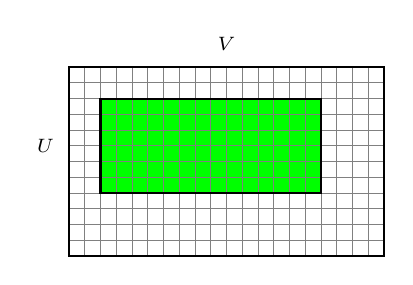
\begin{tikzpicture}
    \draw[fill = green] (0.4, -0.4) rectangle (3.2, -1.6);
    \draw[step = 0.2, gray, thin] (0, 0) grid (4, -2.4);
    \draw[black, thick] (0, 0) rectangle (4, -2.4);
    \draw[black, thick] (0.4, -0.4) rectangle (3.2, -1.6);
    \node at (-0.3, -1.) {\scriptsize $U$};
    \node at (2, 0.3) {\scriptsize $V$};
\end{tikzpicture}

            \end{center}
        \end{column}

		\begin{column}{0.48\textwidth}
            \begin{center}
                Triangle (real) dag:
                \vspace{0.2cm}
                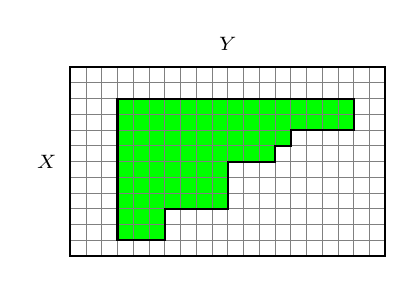
\begin{tikzpicture}
    \draw[fill = green] (0.6, -0.4) -- (3.6, -0.4) -- (3.6, -0.8) -- (2.8, -0.8) -- (2.8, -1) --
    	(2.6, -1) -- (2.6, -1.2) -- (2, -1.2) -- (2, -1.8) -- (1.2, -1.8) -- (1.2, -2.2) -- (0.6, -2.2) --
        cycle;
    \draw[step = 0.2, gray, thin] (0, 0) grid (4, -2.4);
    \draw[black, thick] (0.6, -0.4) -- (3.6, -0.4) -- (3.6, -0.8) -- (2.8, -0.8) -- (2.8, -1) --
    	(2.6, -1) -- (2.6, -1.2) -- (2, -1.2) -- (2, -1.8) -- (1.2, -1.8) -- (1.2, -2.2) -- (0.6, -2.2) --
        cycle;
    \draw[black, thick] (0, 0) rectangle (4, -2.4);
    \node at (-0.3, -1.2) {\scriptsize $X$};
    \node at (2, 0.3) {\scriptsize $Y$};
\end{tikzpicture}

            \end{center}
		\end{column}
	\end{columns}
\end{frame}


\begin{frame}{$\KWm$ relation (Karchmer, Wigderson 1990)}

    $f:\{0, 1\}^n \to \{0, 1\}$ is a monotone partial function
    
    \begin{itemize}
        \item Alice receives $u \in f^{-1}(1)$, Bob receives $v \in f^{-1}(0)$;
        \item goal is to find $i$ such that $u_i = 1 \land v_i = 0$.
    \end{itemize}

    \pause

    \begin{theorem}[Razborov 95; Pudl{\'{a}}k 10; S 17]
        Monotone boolean circuit for $f$ of size $S$ $\Leftrightarrow$ rectangle dag protocol of size $S$
        for the $\KWm_f$ relation.
    \end{theorem}

    \pause

    \begin{theorem}[Hrube{\v{s}} Pudl{\'{a}}k 17]
        Monotone real circuit for $f$ of size $S$ $\Leftrightarrow$ triangle dag protocol of size $S$
        for the $\KWm_f$ relation.
    \end{theorem}
\end{frame}


\begin{frame}{Canonical search problem $\Search_{\varphi}$ (Lov{\'{a}}sz et al. 1994)}
    
    $\varphi(x, y)$ is an unsatisfiable CNF formula:
    \begin{itemize}
        \item Alice receives a substitution to the variables $x$, Bob receives a substitution to the
            variables $y$;
        \item goal is to find a clause $C \in \varphi$ that is unsatisfied by this substitution.
    \end{itemize}

    \pause

    \begin{theorem}[Kraj{\'{\i}}{\v{c}}ek 95; S 17]
        If there a proof of $\varphi$ in $CC_{\log(n)}$ proof system then there is a rectangle dag protocol for
        $\Search_{\varphi}$ of size $\poly(n) S$.
    \end{theorem}

    Resolution, $\CP^*$, $\dots$ are $CC_{\log(n)}$ proof systems.

    \pause
    
    \begin{theorem}[S 17]
        If there a proof of $\varphi$ in $\CP$ proof system then there is a triangle dag protocol for
        $\Search_{\varphi}$ of size $\poly(n) S$.
    \end{theorem}
\end{frame}


\begin{frame}{Results}
    \begin{theorem}
        Let $m = n^{256}$. For any relation $S \subseteq \{0,1\}^n \times \mathcal{O}$, size of boolean
        (real) dag communication protocol of $S \circ \Ind_m^n$ is at least $n^{\Theta(w(S))}$, where
        $w(S)$ is the width of decision dag for $S$.
    \end{theorem}
\end{frame}
